\chapter{Zweites Kapitel}

\section{Fließtext mit Verweis und Abbildung}

%
%   Verweis im Text bei Nennung des Autors (citet) oder in Klammern (citep) 
%
Dies ist der Grund, so \citet{jurafsky2009}, warum sich die meisten Übersetzungsbüros 
für diese Art der Übersetzung entscheiden.
Der Übersetzungsservice (Abbildung~\ref{fig:bildlabel1}) wird von einem Team von 
Fachleuten \citep[S. 3]{mikolov2013} mit langjähriger Erfahrung im Bereich der 
Übersetzungswissenschaft und des Dolmetschens durchgeführt.

%
%   Grafik einfügen
%
\begin{figure}[htbp]
\centering
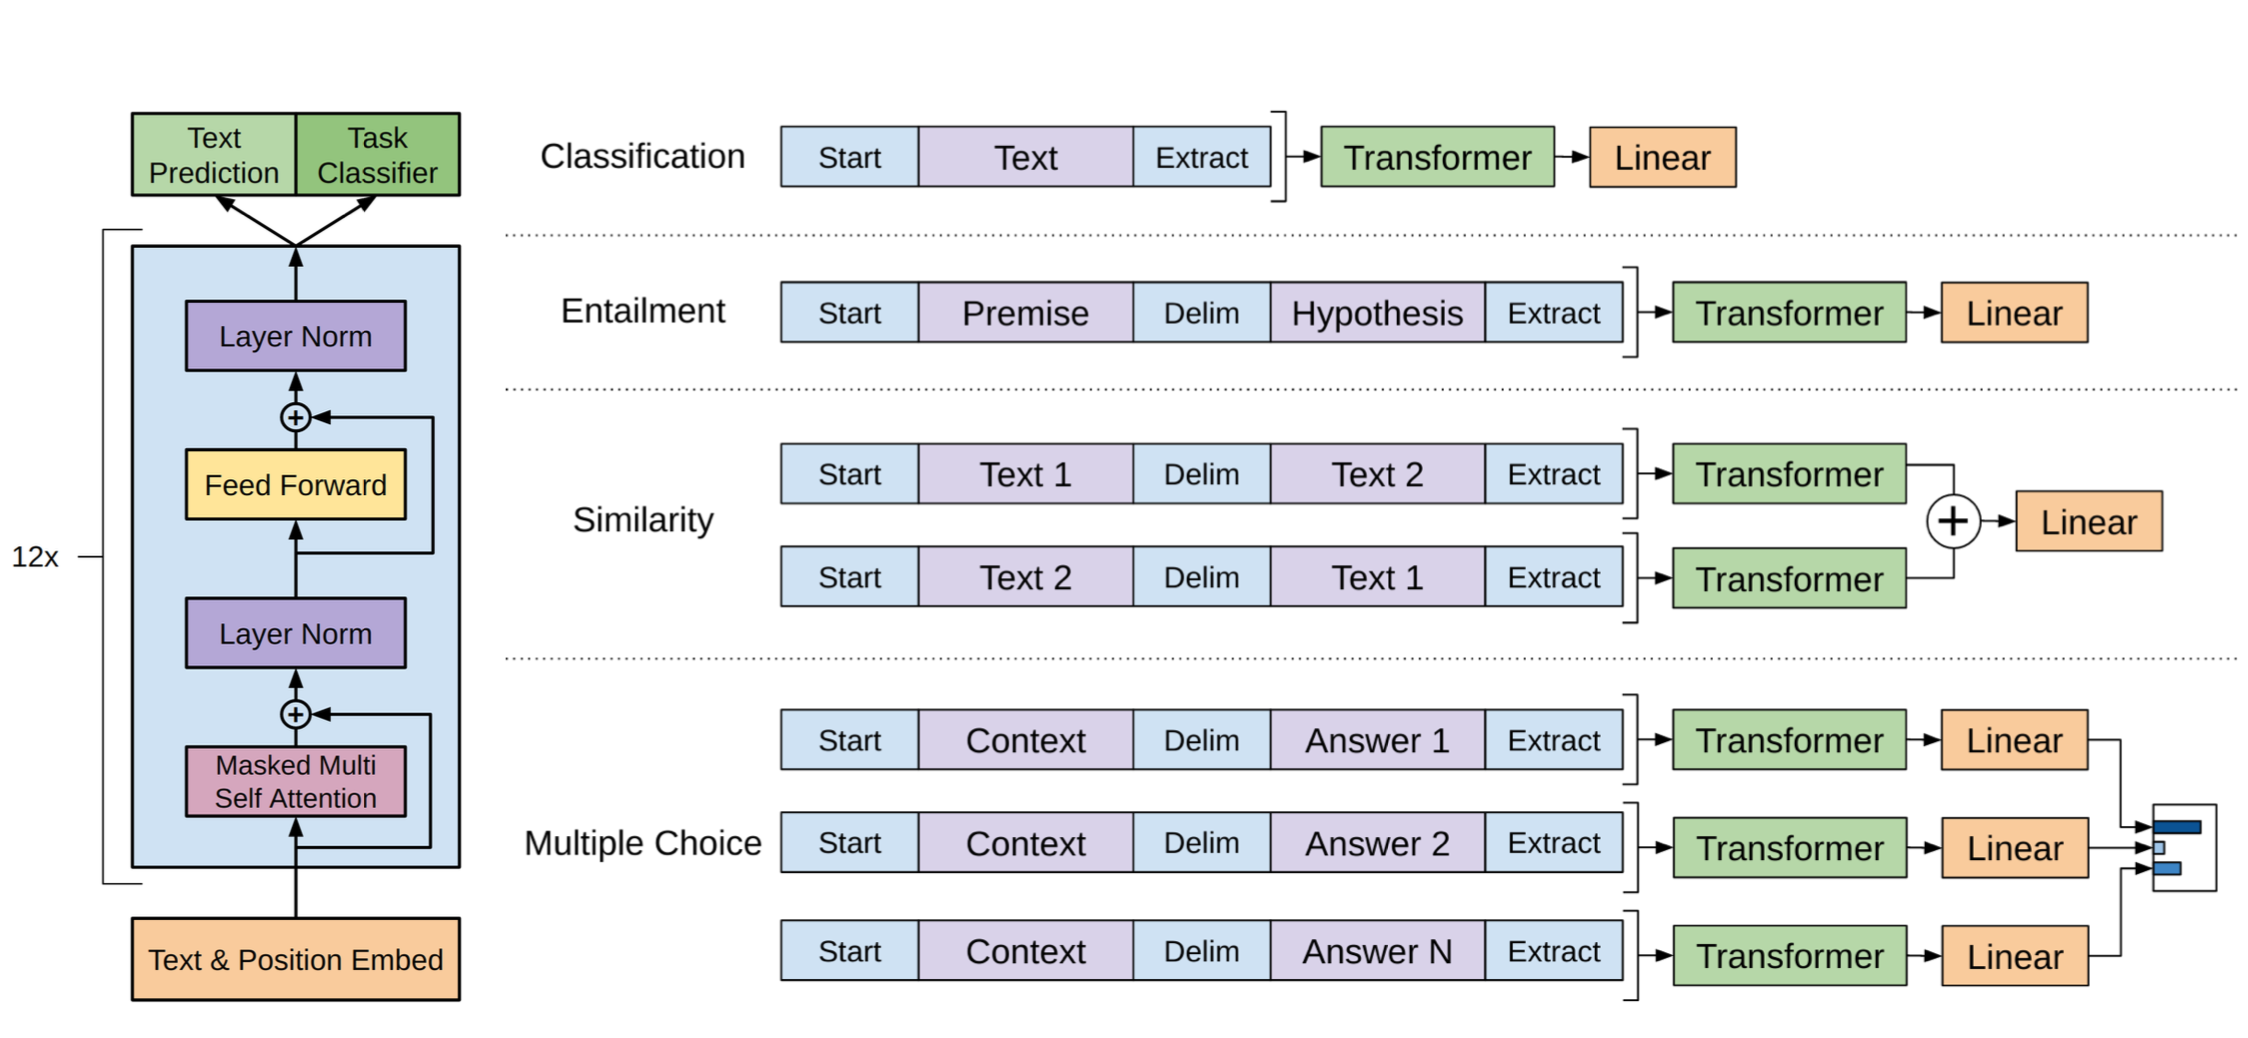
\includegraphics[width=0.5\textwidth]{gpt-model-open-ai-2018}
\caption{GPT-Modell} 
\label{fig:bildlabel1}
\end{figure}

Das Internet ist ein sehr komplexes System, aber es ist sehr leicht zu verstehen, warum es so viele Möglichkeiten gibt, dieses System zu nutzen, obwohl es viele verschiedene Möglichkeiten hat, diesen Prozess zu automatisieren, nämlich die Übertragung von Daten zwischen Computern und Servern, sowie die Verteilung von Nachrichten zwischen den Computern, also zwischen dem PC und dem Server (das heißt, er kann sich auf eine bestimmte Art und Weise mit diesen Computern verbinden und diese Daten an andere Computer weiterleiten, anstatt sie direkt auf den PC zu übertragen).

%
%   Grafik einfügen
%
\begin{figure}[htbp]
\centering
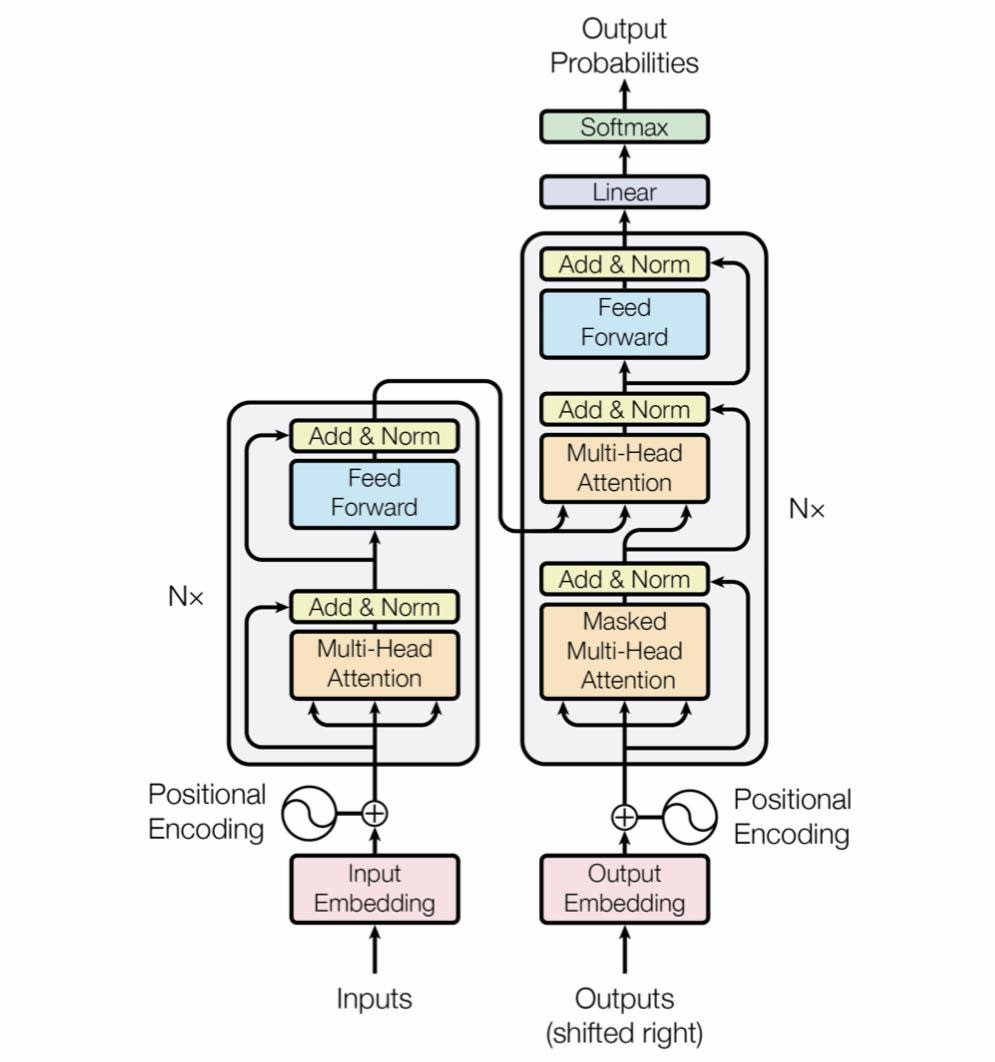
\includegraphics[width=0.8\textwidth]{gpt2}
\caption{Der Titel der Abbildung} 
\label{fig:bildlabel2}
\end{figure}

Das Übersetzungsbüro (Abbildung~\ref{fig:bildlabel1}) bietet eine breite Palette von Übersetzungsdienstleistungen an, angefangen bei der Auswahl der Sprachen für die jeweilige Sprache, bis hin zur Erstellung von Übersetzungen für jede Sprache und für jedes Format, das für den jeweiligen Kunden am besten geeignet ist (z. B. Chinesisch, Koreanisch, Arabisch, Thai, Vietnam, usw.).

\section{Abkürzung und Anführungszeichen im Text}

%
% Beispiel Abkürzung
%
Eine Abkürzung ist z.B. \gls{etc}, die im Abkürzungsverzeichnis erklärt wird. Beim erneuten Vorkommen der Abkürzung \gls{etc} wird nur noch diese gedruckt.

%
% Beispiel Anführungszeichen
%
Anführungszeichen kann man entweder \enquote{so} erstellen oder mit UTF8-encodierter Quelldatei auch „so“.
Der Computer ist ein \enquote{Computer}, in dem sich der \enquote{Benutzer} befindet und der sich mit ihm in \enquote{Verbindung} setzt, so dass er von ihm gesteuert werden kann, ohne dass ihm der Zugang zum Computer verwehrt wird (wenn er das nicht tut, ist er gezwungen, ihn auszuschalten, da er die Kontrolle über das Computersystem hat), oder er kann sich selbst nicht an einen Computer anschließen, indem er sich an eine beliebige andere Maschine anschließt (es ist nicht möglich, ein Programm zu installieren, welches die ganze Maschine ausführt, selbst wenn es nicht funktioniert);

\section{Beispiel Fußnote}

%
%   Beispiel Fußnote mit Referenz
%   Die Referenz A muss in bib.bib enthalten sein
%
Dieses Programm\footnote{vgl. \cite{jurafsky2009}}
ist sehr einfach zu bedienen, da es die Möglichkeit\footnote{Dies ist eine Fußnote ohne Referenz}
bietet, eine Reihe von Funktionen zu implementieren, von denen die meisten für die Programmierung von Programmiersprachen geeignet sind.

\section{Beispiel Tabelle}

Der Text wird dann in ein anderes Format (siehe in Tabelle~\ref{tab:tabellenlabel1}) 
konvertiert, das dann als die Originaldatei bezeichnet wird, wenn der Text in einer anderen Form vorliegt, als das Original, wobei die ursprüngliche Übersetzung unverändert bleibt, bis die originale Übersetzung erneut verwendet wird.

%
%   Beispiel Tabelle
%
\begin{table}[htbp]
\centering
\begin{tabular}{l|l|l|l}
SpalteA & SpalteB & SpalteC & SpalteD \\
\midrule
A1 & B1 & C1 & D1 \\
A2 & B2 & C2 & D2 \\
A3 & B3 & C3 & D3
\end{tabular}
\caption{Beispiel einer Tabelle}
\label{tab:tabellenlabel1}
\end{table}

Sie ist in der Lage, in einem einzigen Arbeitsschritt die Sprache zu programmieren und zu übersetzen, ohne dass es sich dabei um eine maschinelle Übersetzung handelt, die sich auf die Übersetzung der Originalsprache bezieht, wie sie von den meisten anderen Übersetzungsdienstleistern verwendet wird (z.B. von Google, Yahoo, etc.).
Die automatische Übersetzung von Quelltext in die Zielsprache ist eine der am häufigsten verwendeten Formen der maschinellen Übersetzung, wenn es um die Übertragung von Text in eine andere Sprache geht, d.h. eine Übersetzung in mehrere Sprachen, z. B. Englisch, Französisch, Deutsch, Italienisch, Spanisch, Portugiesisch, Russisch, Niederländisch, Polnisch, Schwedisch, Dänisch oder Norwegisch (oder umgekehrt).
